\documentclass[12pt]{article}
\usepackage{amsmath}
\usepackage{graphicx}
\begin{document}
\title{Photometry and images from smart telescopes}

\section{Introduction}

Smart telescopes, such as the SeeStar S50 (etc...) are very popular and eliminate
most of the barriers to entry into astrophotography. For a relatively modest price
a smart "telescope" is the optical componenets of a telescope, a one-shot-color
CMOS sensor, a housing, and a basic trtipod. The device takes regular, short
exposures, e.g. 10 seconds for the SeeStar S50, plate solves each exposure and
builds a stacked color image on the fly. Image taking continues until the user
stops it. The user has the option of saving only the stacked color image or the
stacked image and also of the subframes that went into the stack.

While manufacturers of these devices have focused on their use for
astrophotography, the CMOS sensors in them are adequate for performing aperture
photometry on the stars in the image. The devices typically have a wide field
of view so as to maximize the visual impact of the images they take. That implies
a fairly large pixel scale of 1-2 arcsec/pixel with a stellar full-width at half maximum (FWHM) of 3-5 pixels.

The combination of under-resolved stars and a Bayer array on the image sensor is a challenge. The traditional
approach of separating the one-shot color image into three separate lower-resolutions images, one for each
of the three color channels, will lead to severely under-resolved stars. In this paper we present an
alternative method based on applying masks to the image to select one color at a time.

In Section \ref{sec:method} we describe our methods for performing photometry on
both individual subframes and stacked images. Section XXX presents the application of these methods to a few variable stars and smart telescopes. Finally, Section YYY does SOMETHING OR ANOTHER.

\section{Methods} \label{sec:method}

There are two distinct tasks that need to be handled for each of the images: source detection/centroiding and
aperture photometry. The latter is fairly straightforward once source locations have been identified, but
the former requires some care because of the presence of the Bayer array.

\subsection{Source detection and centroid location}
The presence of the Bayer array means that the background level in each color may not be uniform
across colors. An example is shown in the left column of Figure \ref{fig:color-cutout}. The image is
of the variable star T CrB taken with a SeeStar S50, relatively early in the evening when the sky
still had a significant blue cast.

Attempting to perform source detection on the raw image will lead to large number of spurious detections because the blue pixels are so much brighter than the red and green pixels. To mitigate this problem, we apply what we call Bayer balancing to the image. To Bayer balance the image, we scale each color channel's data so that the standard deviation of each color channel to match the standard deviation of the entire image, ignoring color, and then adjust the mean of each color channel to match the mean of the entire image. The result is shown in the right column of Figure \ref{fig:color-cutout}. The background level is now more uniform across colors, and source detection can be performed on the Bayer balanced image without a large number of spurious detections. TODO: DOES THIS NEED A PLOT?

\begin{figure}
    \centering
    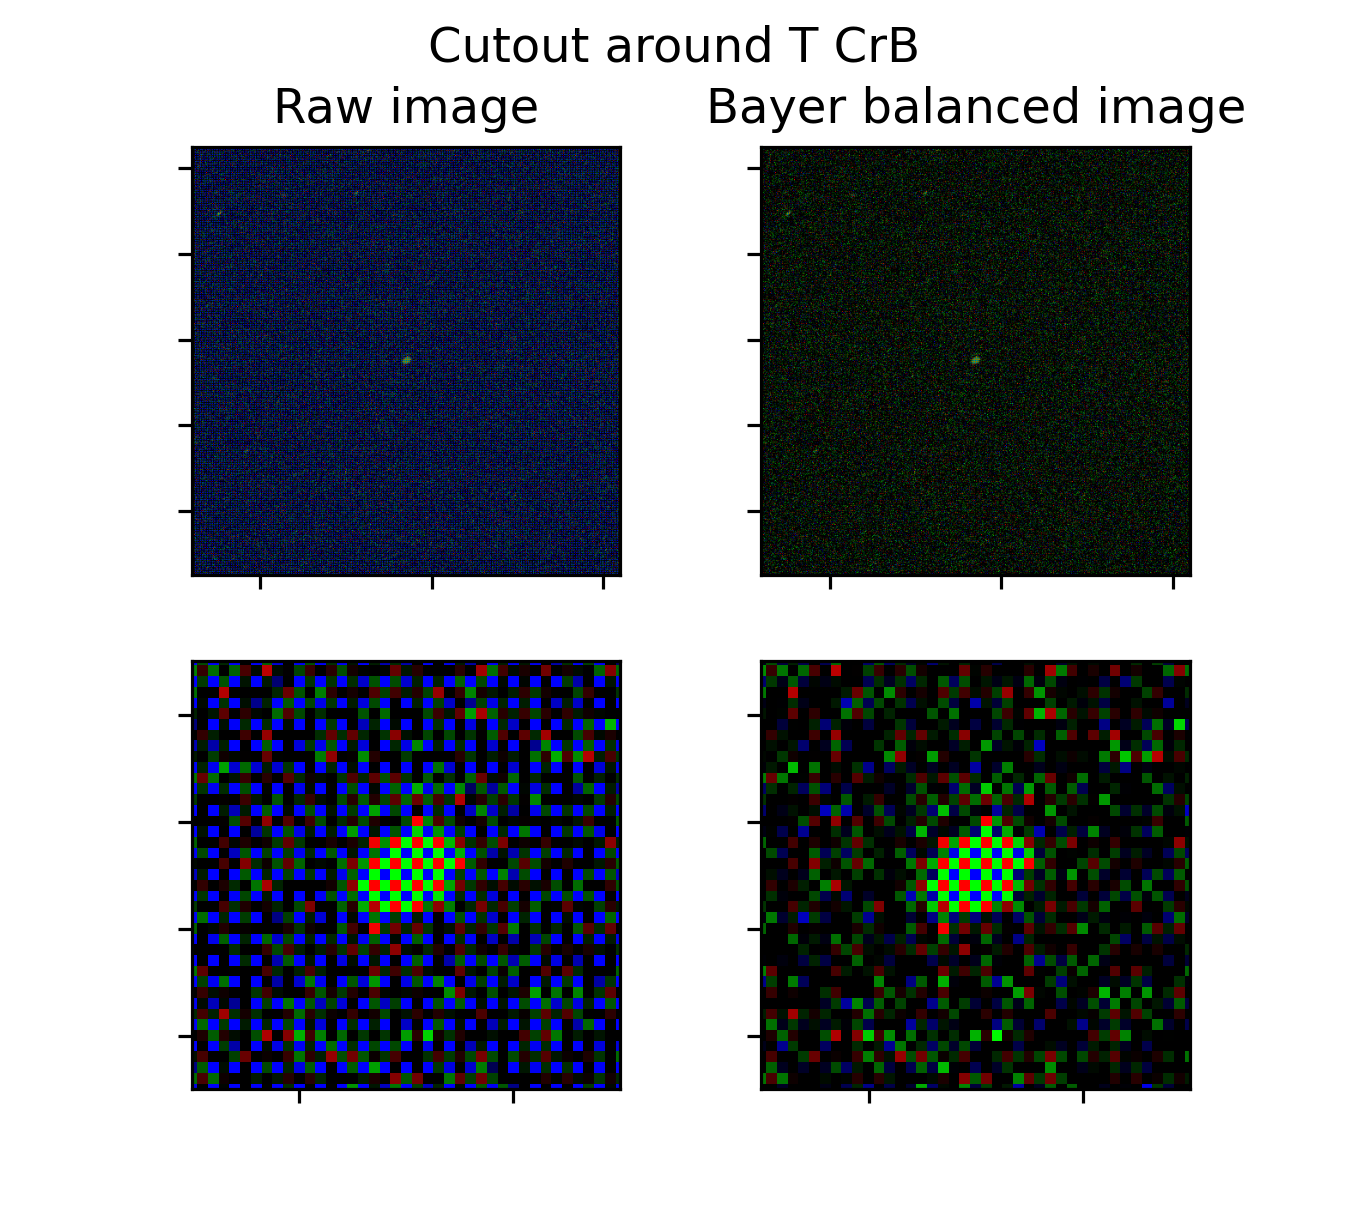
\includegraphics[width=0.8\textwidth]{color-cutout.png}
    \caption{Cutout around T CrB showing the effect of the Bayer array on the background level. The left column shows the raw image, while the right column shows the result of applying a Bayer balance to the image. The top row shows a wide cutout, while the bottom row shows a zoomed-in cutout.}
    \label{fig:color-cutout}
\end{figure}
\end{document}
